% The non-floating teaser stays immediately below the title, above the abstract.
\vspace{-14pt}
\begin{center}
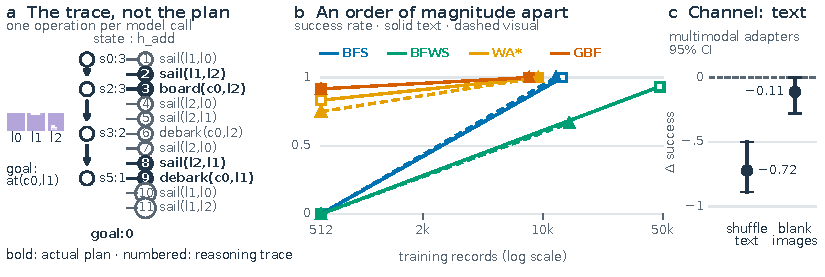
\includegraphics[width=\textwidth]{figures/fig_teaser.pdf}
\captionof{figure}{\textbf{Learning search from traces at two levels.} (a)~We supervise every operation of the BFS search on a ferry task, not only the four-operator plan (bold). (b)~Executing BFS and BFWS fails from a small training set in every observation type and succeeds only with far larger sets, evaluated on separate panels (hollow). (c)~Choosing the next node for GBFS and WA* from images alone beats random valid choices on two held-out panels. (d)~Training on BFWS traces raises FOLIO accuracy above the base model, and training on BFS traces does not.}
\label{fig:teaser}
% Evidence (a): outputs/expanded-study/v1/baseline/episodes/text-state/expanded-final__ferry-compact-915000/bfs-exact_reference.json.gz result.{decision_count 10, expansion_count 7, goal_reached}; plan reconstructed from parent links and asserted equal to outputs/expanded-study/v1/panel-v2/views/ferry-compact-915000/scenes/catalog.json.gz path_bindings[1].supplied_actions (4 operators); unlabelled/state-000000.png unchanged.
% Evidence (b, small set): docs/experiments/expanded-study/synthesis-v1/baseline-summary.csv process_sft rows {bfs,best_first_width} x {text,visual,multimodal}-state, 0/24 each; 512 records per outputs/matched_modalities/{v3,v5}/training/*/{bfs,best_first_width}/report.json train_records.
% Evidence (b, larger development runs): text BFS 12,994 (data/bfs_pilot_v6/ms-swift-process/manifest.json counts.train) -> 1.0 (docs/experiments/deadline-study/prior-evidence.json historical_bfs_stages v8); text BFWS 47,780 (data/bfws_phase_v1/corpus-release/training/manifest.json) -> 14/15 (data/bfws_phase_v1/issue59-distributed-terminal/adjudication-report.json); visual BFS 11,911 -> 75/75 and visual BFWS 14,225 -> 50/75 (outputs/visual_development/issue75-32k-v5/attempt-001/training.json; prior-evidence.json issue75.metrics).
% Evidence (c): outputs/choice-frontier/v4/panels/metrics/analysis.json arms.p2 (held-out 1: 11 tasks x GBFS/WA*) and arms.p2u (held-out 2: 12 tasks) .solved_at_2: learned s17/s29/s71 0.636/0.545/0.682 (mean 0.621) and 0.333/0.208/0.292 (mean 0.278); random 0.036 and 0.017; exact 1.0.
% Evidence (d): docs/experiments/expanded-study/synthesis-v1/transfer-accuracy.csv folio: base 0.600; bfs_text/visual/multimodal 0.600/0.605/0.605; iw_text/visual/multimodal 0.660/0.645/0.645. Report: teaser_v3_report.md.
\end{center}
\vspace{-10pt}

\begin{abstract}
The automated planning community has probed the planning ability of large language models by fine-tuning them on planning-problem corpora, but the training target is almost always the \emph{plan} (i.e., the action sequence a planner returns), rather than the search that found it. Yet classical planning offers many search algorithms, and how well a model learns them from their search traces is still an open question. As embodied agents increasingly plan from what they see, the question extends to vision-language models (VLMs). We fine-tune a VLM on the search traces of four classical algorithms across 15 PDDL domains and study learning at two levels. For breadth-first search (BFS) and best-first width search (BFWS), whose expansion order follows from bookkeeping rules, the model executes the algorithm, writing every step of the search, including where each new node goes in the open list. For greedy and weighted-$A^*$ best-first search, whose order follows the additive heuristic, the model makes the search-control decision, choosing which node to expand next from images of the open nodes, with no heuristic values shown. Execution is learnable but costly: from a small training set the model solves no tasks under either algorithm, and it reaches success of 1.0 for BFS and 0.93 for BFWS only with over an order of magnitude more data. Search control is learnable from images alone: on held-out tasks, the trained VLM solves 0.28 to 0.62 of tasks within twice the reference budget, against at most 0.04 for random valid choices. Training on width-based traces even transfers beyond planning, raising logical-reasoning accuracy on FOLIO from 0.600 to 0.660. Together, these results establish search traces as a practical supervision target for planning research, alongside plans.
\end{abstract}
